\documentclass[a4paper,11pt]{article}

\usepackage[margin=2.4cm]{geometry}
\usepackage{amsmath,amssymb}
\usepackage{booktabs}
\usepackage{array}
\usepackage{enumitem}
\usepackage{float}
\usepackage{graphicx}
\usepackage{xcolor}
\usepackage{xurl}
\usepackage{hyperref}
\usepackage{caption}

\graphicspath{{figures/}}
\hypersetup{
  colorlinks=true,
  linkcolor=blue!60!black,
  citecolor=blue!60!black,
  urlcolor=blue!60!black
}
\setlist[itemize]{nosep,leftmargin=1.8em}
\setlist[enumerate]{nosep,leftmargin=1.8em}

\title{\textbf{Technical Report on Constraining $\gamma$ with 190 MeV/u Polarized-Deuteron Breakup}}
\author{Baiting Tian}
\date{June 11, 2026}

\begin{document}
\maketitle

\section*{Data Scope}

\begin{itemize}
  \item Local repository: \texttt{/home/tian/workspace/dpol/smsimulator5.5}
  \item NEBULA-Plus reconstruction sample: {\footnotesize\path{/home/tian/workspace/sshDir/spana03/Dpol_smsimulator/data/reconstruction/nebulaplus_nn_joint_20260609_012854}}
  \item Folding diagnostic tables: \texttt{checks/observables/folding\_diagnostics/}
  \item Figures used in this report: \texttt{docs/reports/gamma\_constraint\_20260611/figures/}
\end{itemize}

\section*{Executive Summary}

The current simulation and reconstruction sample support the following statements.

\begin{enumerate}
  \item For Sn124, the folded visible-window observable with the tight selection and $|p_{x,n}|<60$ MeV/$c$ still keeps a clear dependence on $\gamma$. In y-pol, the folded reconstructed $R$ changes from about $12.48$ to $4.99$ when $\gamma$ changes from 0.5 to 0.8. In z-pol, it changes from about $6.38$ to $0.56$.
  \item For a 15 mm diameter Sn124 target made from the 1.2 g inventory, a beam intensity of $1.0\times10^7$ pps, and 16 h of beam time, the current planning anchor gives enough statistics even after applying a conservative usable-event survival factor from the full simulation: about $2.75\times10^5$ usable $R$ events for y-pol and $1.88\times10^6$ for z-pol.
  \item The hardest adjacent model separation in the current grid is y-pol $g070 \to g080$. A purely statistical 3$\sigma$ separation needs only about $2.8\times10^3$ usable $R$ events. Statistics are therefore not the leading limitation.
  \item The main risk is systematic, not statistical. The new diagnostics show the detector folding explicitly: event-selection survival, neutron $p_x$--$p_y$ efficiency, $p_{x,n}$ and $\Delta p_x$ response matrices, reaction-plane migration, sign migration, and the final $R$ ladder. Truth-level $R$ and reconstructed $R$ are not the same quantity; the robust strategy is to fold every theory point through the same Geant4 and reconstruction chain before comparing it with data.
  \item The PDC geometry is treated as the final effective 69 deg configuration. The NEBULA-Plus macro executes the base geometry first, then explicitly sets the PDC angle to 69 deg and calls \texttt{Update}. The 65 deg message in the logs is an earlier setting that is overwritten.
\end{enumerate}

\section{Coordinate, $p_x$, and Reaction-Plane Conventions}

The lab frame is the Geant4/SAMURAI world frame used by the NEBULA-Plus macro: $+Z$ points downstream along the nominal beam direction, $+Y$ is vertical, and $+X$ is the horizontal dispersive direction shown in the event-display projections below. The target/input frame is the frame of the generated or reconstructed target momentum. Unless a label explicitly says ``lab'', $p_x$ in this report means $p_x^{\mathrm{tgt}}$, i.e. the target-frame component used for the $p_{x,n}$ fiducial cuts and response plots.

The target angle is $\theta_{\mathrm{tgt}}=3^\circ$. In the Geant4 primary generator, a particle is started from the target center and the input target-frame direction is rotated by $-\theta_{\mathrm{tgt}}$ about lab $Y$:
\[
  \mathbf p^{\mathrm{lab}} =
  R_y(-\theta_{\mathrm{tgt}})\,\mathbf p^{\mathrm{tgt}} .
\]
Therefore positive target-frame $p_x$ means an initial component toward lab $+X$ before the common target-angle rotation. For the simple $p_y=0$ sign checks,
\[
  p_x^{\mathrm{lab}}
  =
  p_x^{\mathrm{tgt}}\cos\theta_{\mathrm{tgt}}
  -
  p_z^{\mathrm{tgt}}\sin\theta_{\mathrm{tgt}} ,
\]
using the same rotation convention as the simulation.

\begin{figure}[H]
  \centering
  \begin{minipage}{0.49\linewidth}
    \centering
    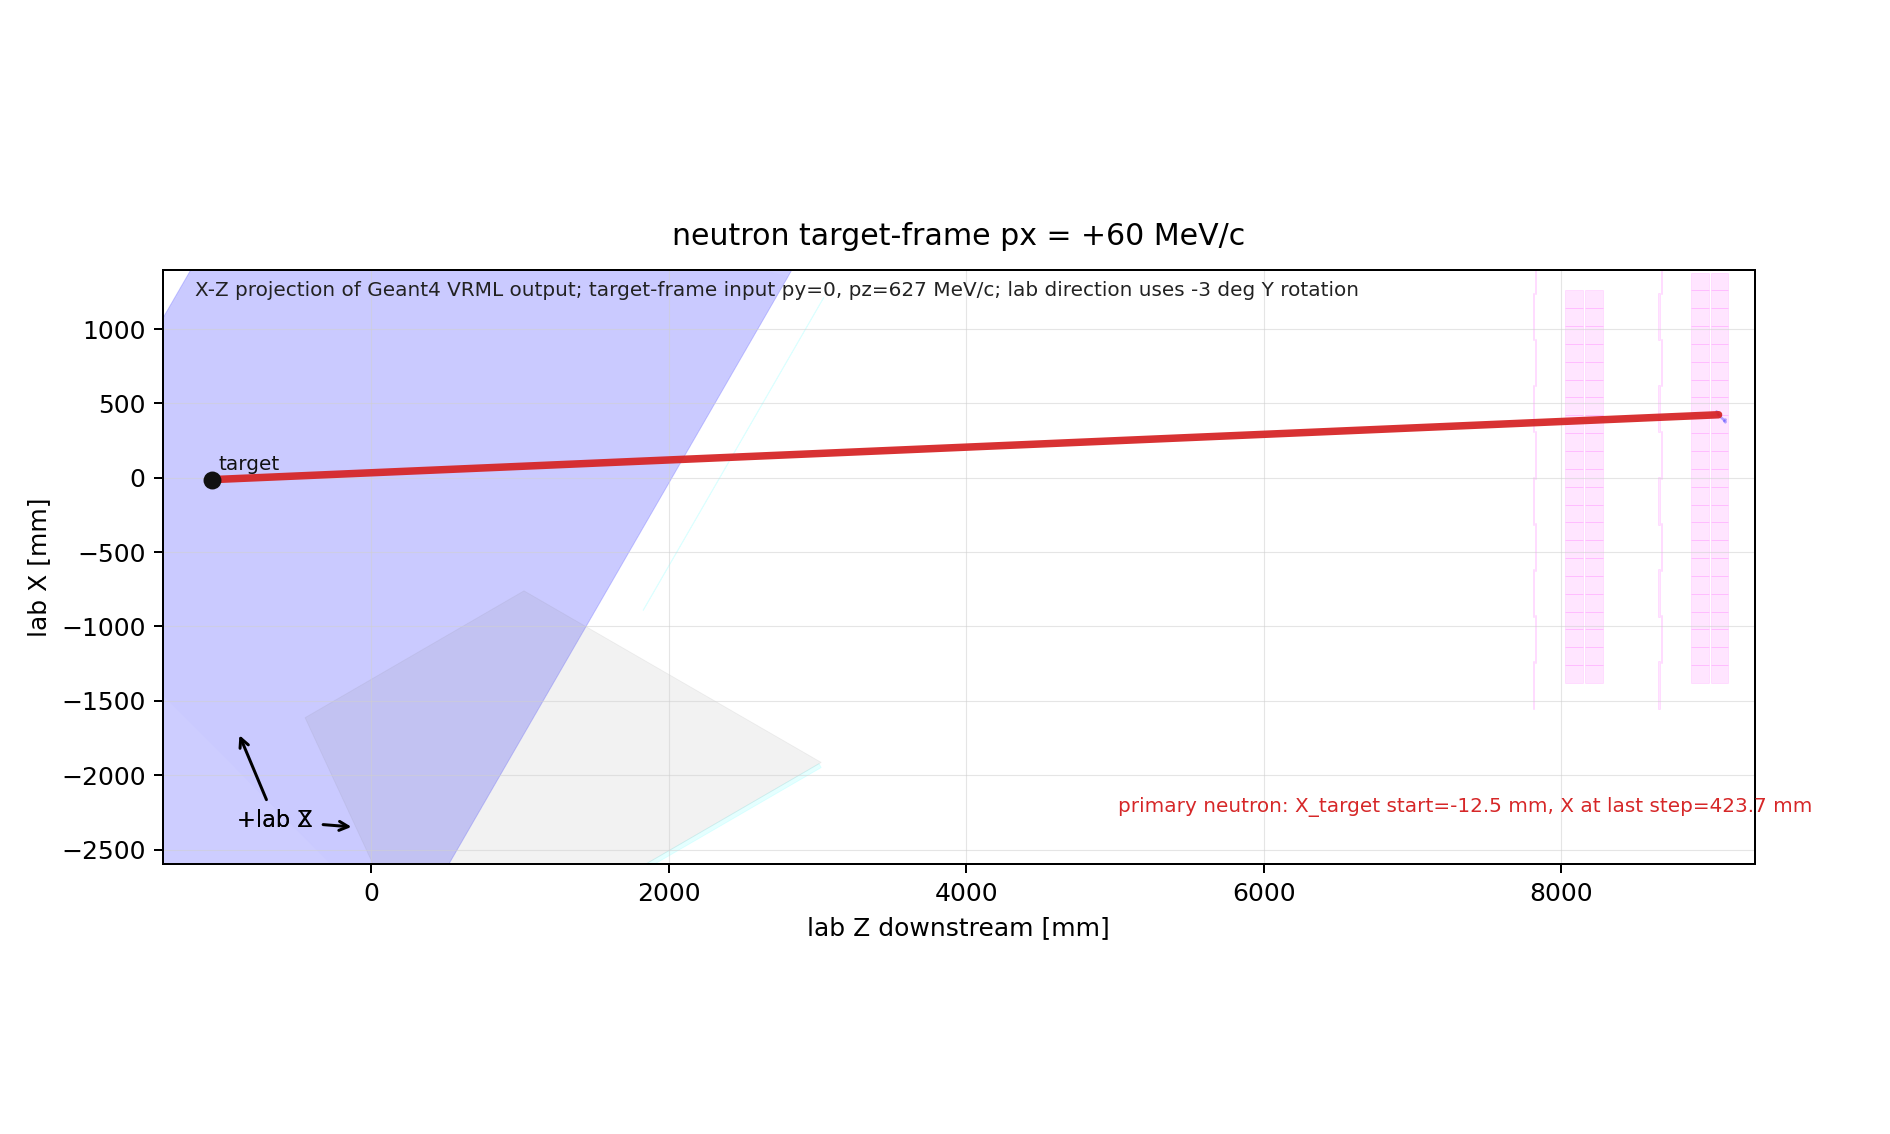
\includegraphics[width=\linewidth]{px_sign_geant4/neutron_px_plus60.png}
  \end{minipage}
  \hfill
  \begin{minipage}{0.49\linewidth}
    \centering
    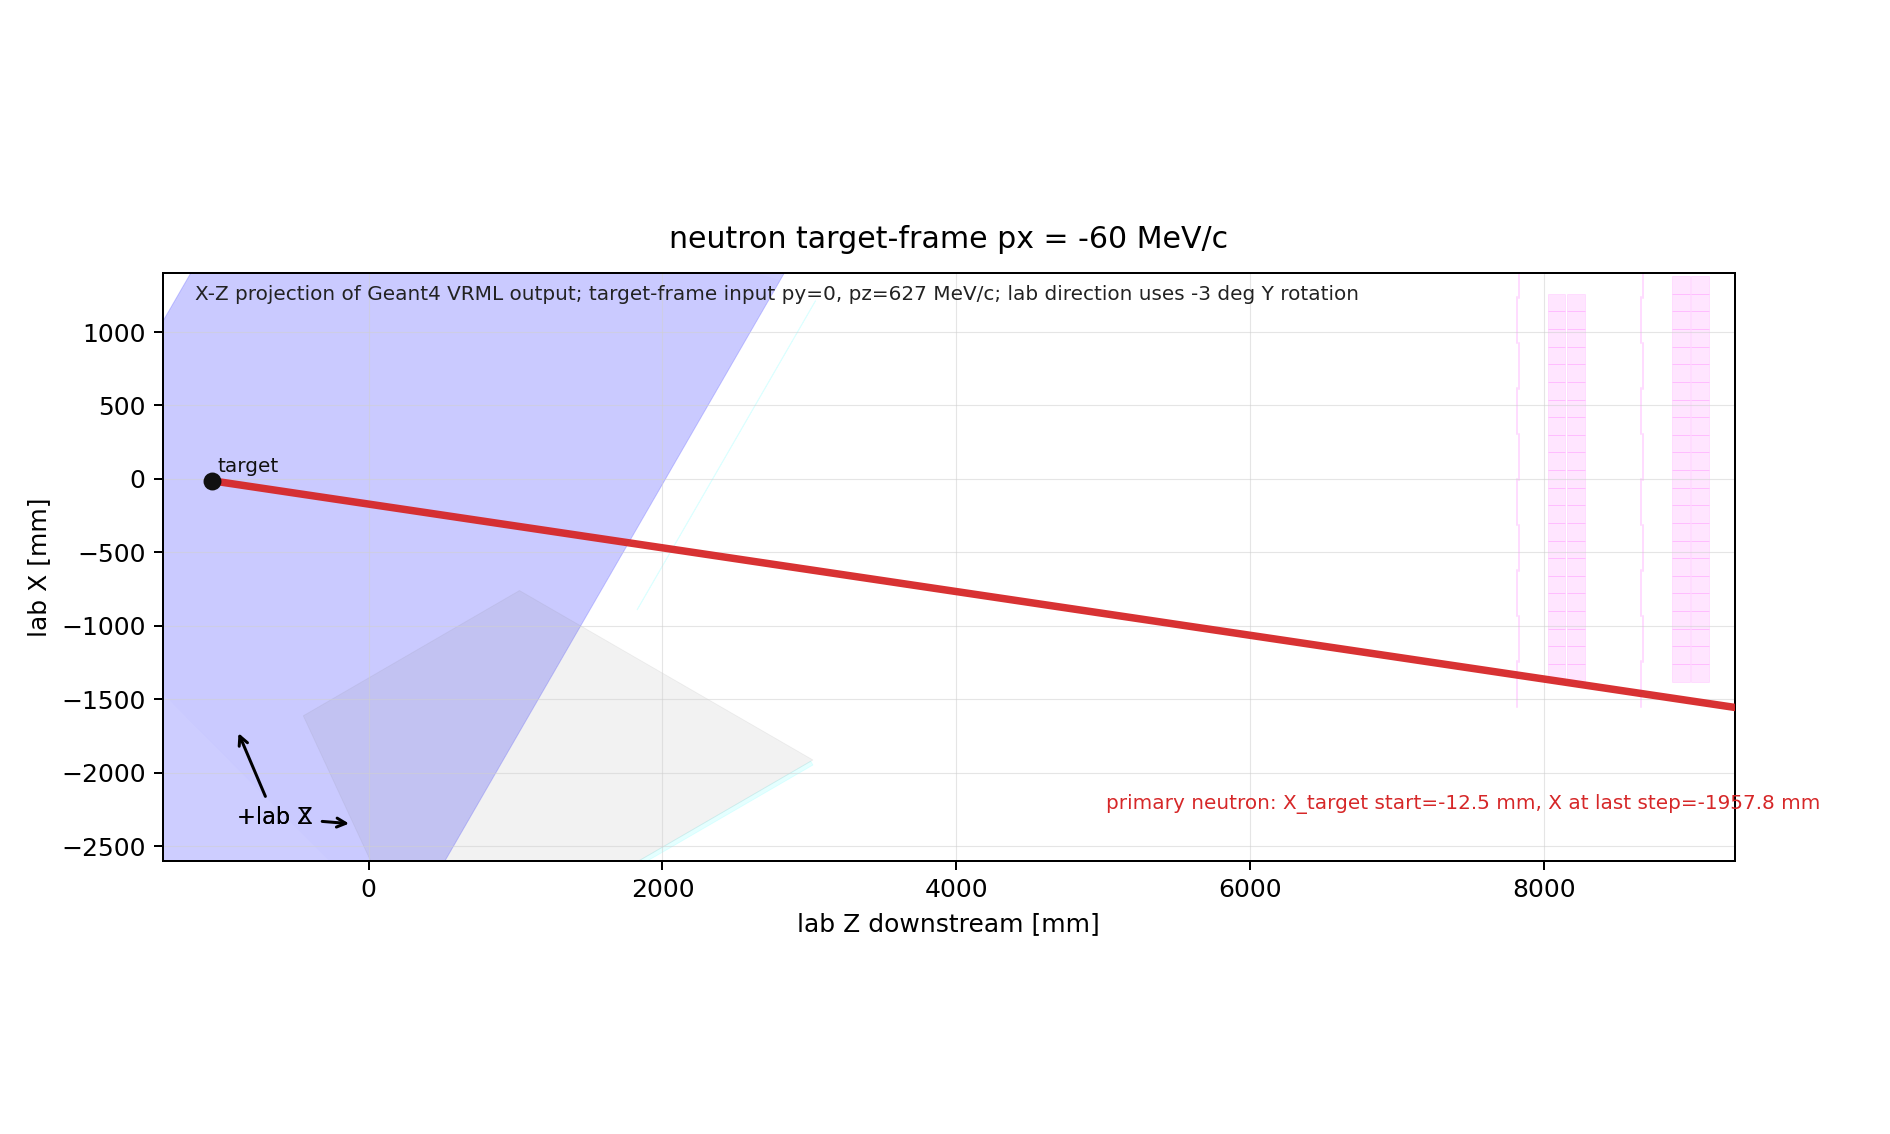
\includegraphics[width=\linewidth]{px_sign_geant4/neutron_px_minus60.png}
  \end{minipage}
  \caption{Geant4 VRML-to-PNG projections for target-frame neutron $p_x=\pm60$ MeV/$c$, with $p_y=0$ and $p_z=627$ MeV/$c$. The horizontal axis is lab $Z$ downstream; the vertical axis is lab $X$. Positive target-frame $p_x$ trends toward lab $+X$ after the $-3^\circ$ target rotation, while negative target-frame $p_x$ trends toward lab $-X$.}
\end{figure}

\begin{figure}[H]
  \centering
  \begin{minipage}{0.49\linewidth}
    \centering
    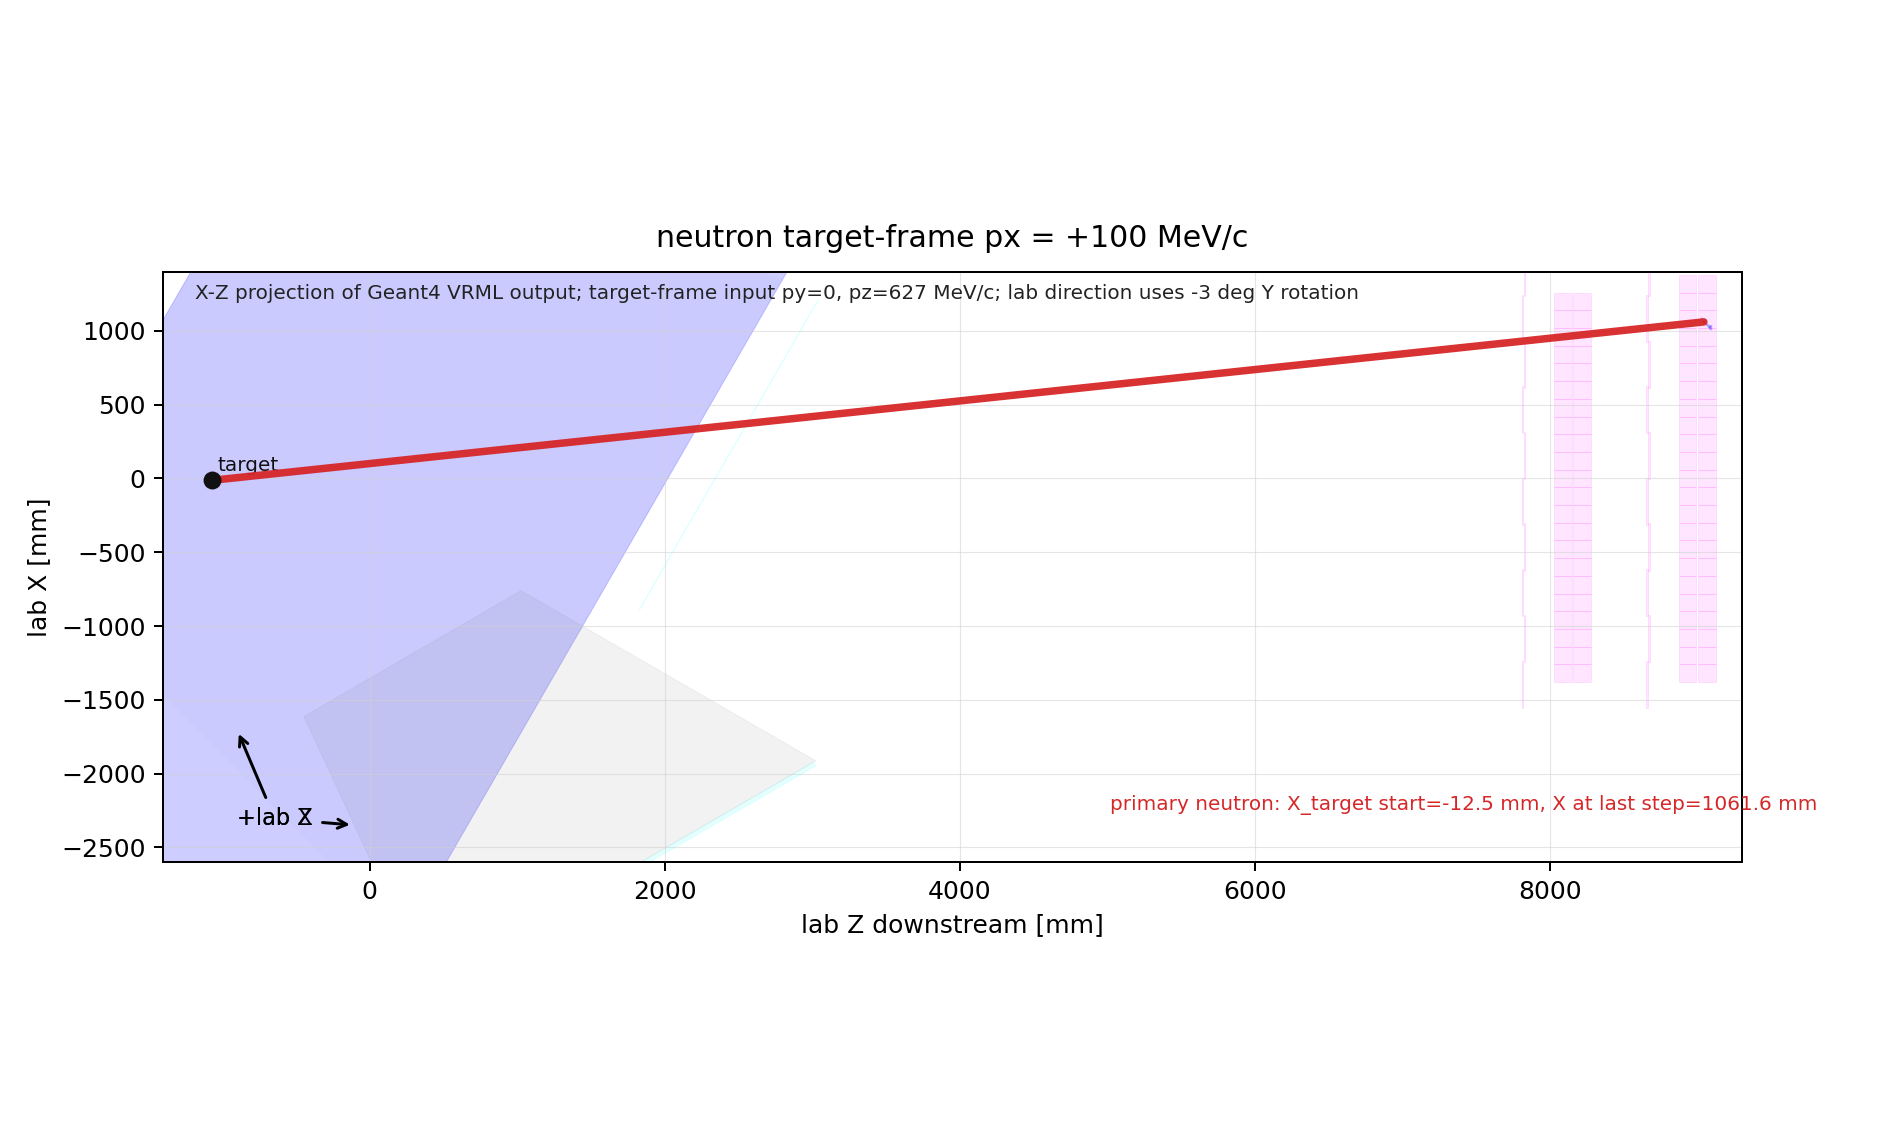
\includegraphics[width=\linewidth]{px_sign_geant4/neutron_px_plus100.png}
  \end{minipage}
  \hfill
  \begin{minipage}{0.49\linewidth}
    \centering
    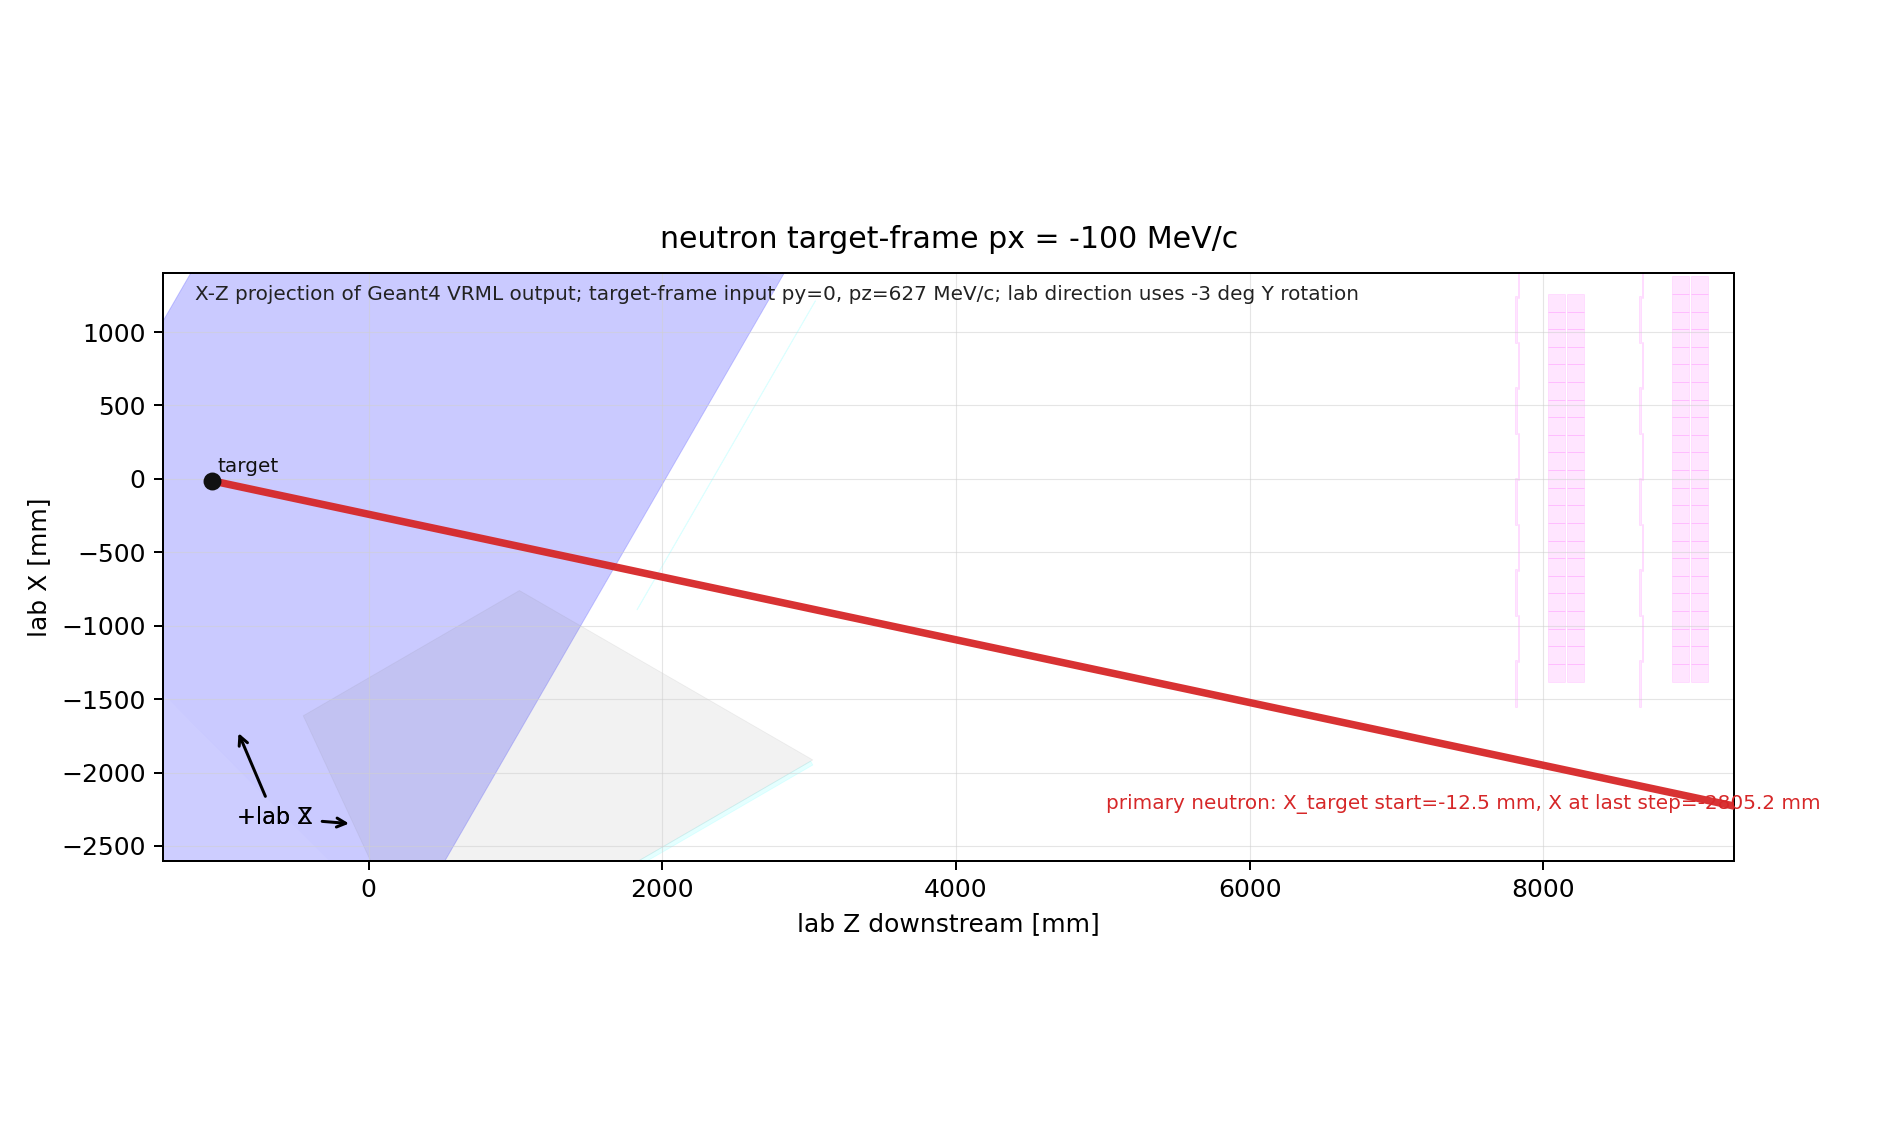
\includegraphics[width=\linewidth]{px_sign_geant4/neutron_px_minus100.png}
  \end{minipage}
  \caption{The same Geant4 sign check for target-frame neutron $p_x=\pm100$ MeV/$c$. The larger $|p_x|$ gives the expected larger lab-$X$ deflection, validating the sign convention used in the reconstructed $p_{x,n}$ plots.}
\end{figure}

Two reaction-plane azimuths must be kept separate. The generator/model angle $b_\phi$ is the reaction-plane azimuth carried by the QMD/event metadata; in the y-pol raw samples it follows the recorded \texttt{rpphi} modulo $2\pi$, while randomized samples carry the randomized plane angle in the event record. This is a truth/model-plane label and is useful for generator checks.

The current folded observable instead uses the event-by-event kinematic plane. Let
\[
  \mathbf k_{\mathrm{out}}
  =
  \mathbf p_p + \mathbf p_n,
  \qquad
  \mathbf k_{\mathrm{out},T}
  =
  (k_{\mathrm{out},x}, k_{\mathrm{out},y}) .
\]
Because $\mathbf k_{\mathrm{in}}$ defines the target-frame beam axis, the azimuth of the $(\mathbf k_{\mathrm{in}},\mathbf k_{\mathrm{out}})$ reaction plane is
\[
  \phi_k
  =
  \operatorname{atan2}
  \left(k_{\mathrm{out},y}, k_{\mathrm{out},x}\right)
  =
  \operatorname{atan2}
  \left(p_{y,p}+p_{y,n}, p_{x,p}+p_{x,n}\right).
\]
If one defines a momentum-transfer vector as $\mathbf q=\mathbf k_{\mathrm{in}}-\mathbf k_{\mathrm{out}}$ instead, the transverse azimuth is shifted by $\pi$; this convention should not be mixed with the current $R$ definition.

The rotation used for $\Delta p_x$ is
\[
  \begin{pmatrix}
    p_x^{\mathrm{rot}} \\
    p_y^{\mathrm{rot}}
  \end{pmatrix}
  =
  R_z(-\phi_k)
  \begin{pmatrix}
    p_x \\
    p_y
  \end{pmatrix}
  =
  \begin{pmatrix}
    p_x\cos\phi_k + p_y\sin\phi_k \\
    -p_x\sin\phi_k + p_y\cos\phi_k
  \end{pmatrix}.
\]
The observable is then
\[
  \Delta p_x
  =
  p_{x,p}^{\mathrm{rot}} - p_{x,n}^{\mathrm{rot}},
  \qquad
  R
  =
  \frac{N(\Delta p_x>0)}{N(\Delta p_x<0)} .
\]

\section{Observable and Physics Logic}

The physics goal is to use the proton--neutron isovector force difference near the target to detect a bias in the final breakup relative momentum. For each event, the transverse reaction-plane direction is defined by
\[
  \phi = \operatorname{atan2}
  \left(
    p_{y,p}+p_{y,n},
    p_{x,p}+p_{x,n}
  \right).
\]
After rotating the proton and neutron momenta into this event plane, the working observable is
\[
  \Delta p_x = p_{x,p}^{\mathrm{rot}} - p_{x,n}^{\mathrm{rot}},
  \qquad
  R = \frac{N(\Delta p_x > 0)}{N(\Delta p_x < 0)}.
\]

The experiment does not observe the truth distribution directly. It observes a folded distribution:
\[
  N_{\mathrm{reco},j}
  =
  \sum_i K_{ji} N_{\mathrm{true},i} + b_j .
\]
Here $K_{ji}$ includes NEBULA/NEBULA-Plus acceptance, resolution, reconstruction efficiency, PDC proton reconstruction, reaction-plane migration, and analysis cuts. In general,
\[
  R_{\mathrm{reco}} \ne R_{\mathrm{truth}}.
\]
This report therefore does not interpret reconstructed $R$ as a direct estimator of truth-level $R$. It instead tests whether $R(\gamma)$ remains separable under a common folded analysis definition.

\section{Most Convincing Current Gamma Sensitivity}

\begin{figure}[H]
  \centering
  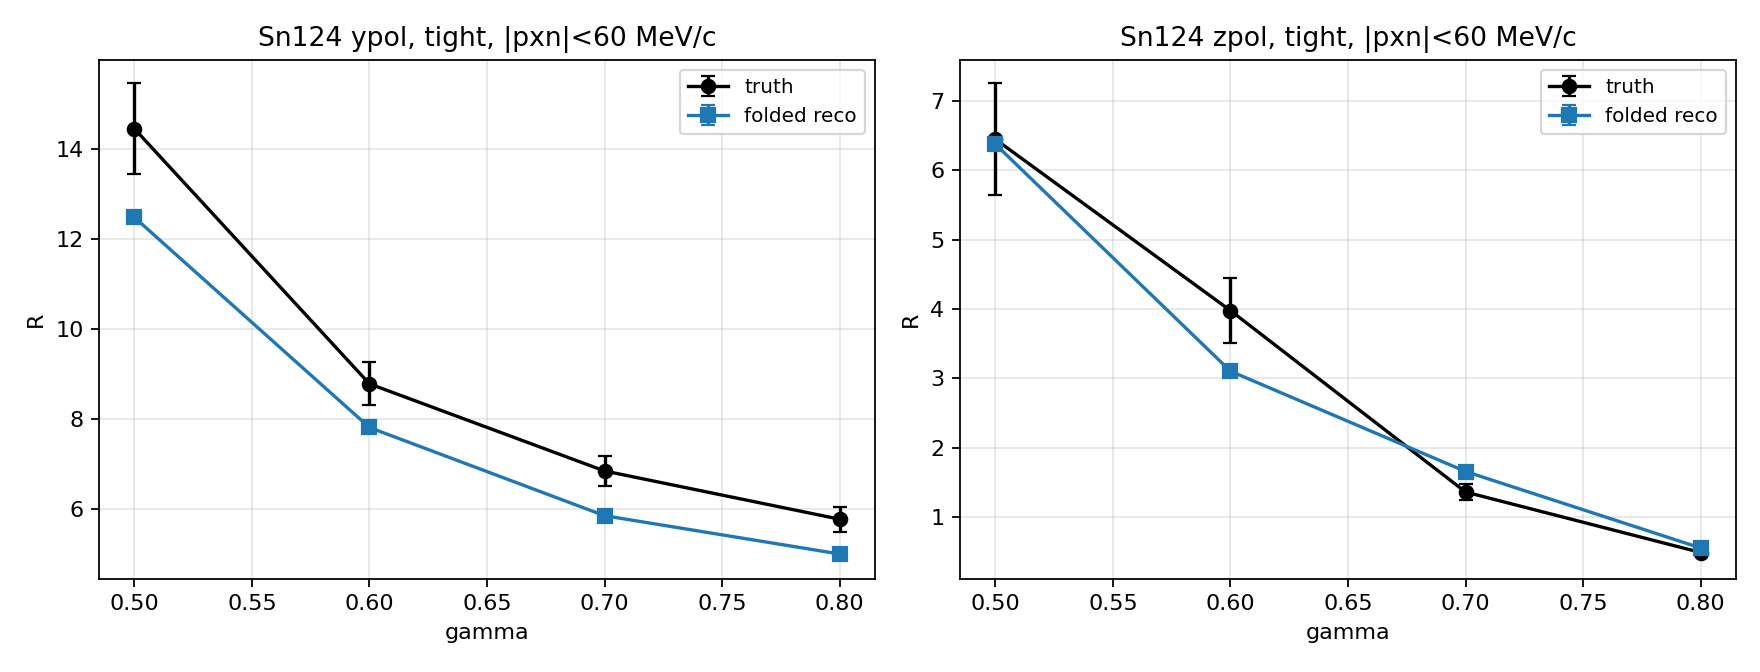
\includegraphics[width=\linewidth]{sn124_tight_px60_r_vs_gamma_expected_stat.png}
  \caption{Truth and folded reconstructed $R(\gamma)$ for Sn124 with the tight selection and $|p_{x,n}|<60$ MeV/$c$.}
\end{figure}

For Sn124 with the tight selection and $|p_{x,n}|<60$ MeV/$c$, the folded reconstructed reaction-plane observable is:

\begin{table}[H]
\centering
\begin{tabular}{llrr}
\toprule
polarization & $\gamma$ & $N_{\mathrm{sim}}$ & $R_{\mathrm{folded}}$ \\
\midrule
y-pol & 0.5 & 2305 & 12.48 \\
y-pol & 0.6 & 2422 & 7.81 \\
y-pol & 0.7 & 2451 & 5.85 \\
y-pol & 0.8 & 2338 & 4.99 \\
z-pol & 0.5 & 354 & 6.38 \\
z-pol & 0.6 & 275 & 3.10 \\
z-pol & 0.7 & 343 & 1.66 \\
z-pol & 0.8 & 478 & 0.56 \\
\bottomrule
\end{tabular}
\end{table}

The important point is not that truth and reconstruction are identical. The important point is that the folded reconstructed curve remains monotonic in the current Sn124 sample, and its separation is much larger than the statistical uncertainty expected for a 16 h run.

\section{Detector Folding Diagnostics}

The detector question is whether the reconstructed observable is still a controlled, calibratable folded observable. The current diagnostics separate the folding into event selection, neutron visible-window efficiency, reconstruction response, reaction-plane migration, and the final $R$ ladder. The available output does not yet contain an independent layer-by-layer proton detector efficiency table; the proton/reaction-plane contribution is therefore evaluated through the PDC-reconstructed event plane, the response matrices, and the \texttt{reco\_truth\_plane} to \texttt{reco\_plane} change in the $R$ ladder.

\subsection{Event selection and visible-window survival}

\begin{figure}[H]
  \centering
  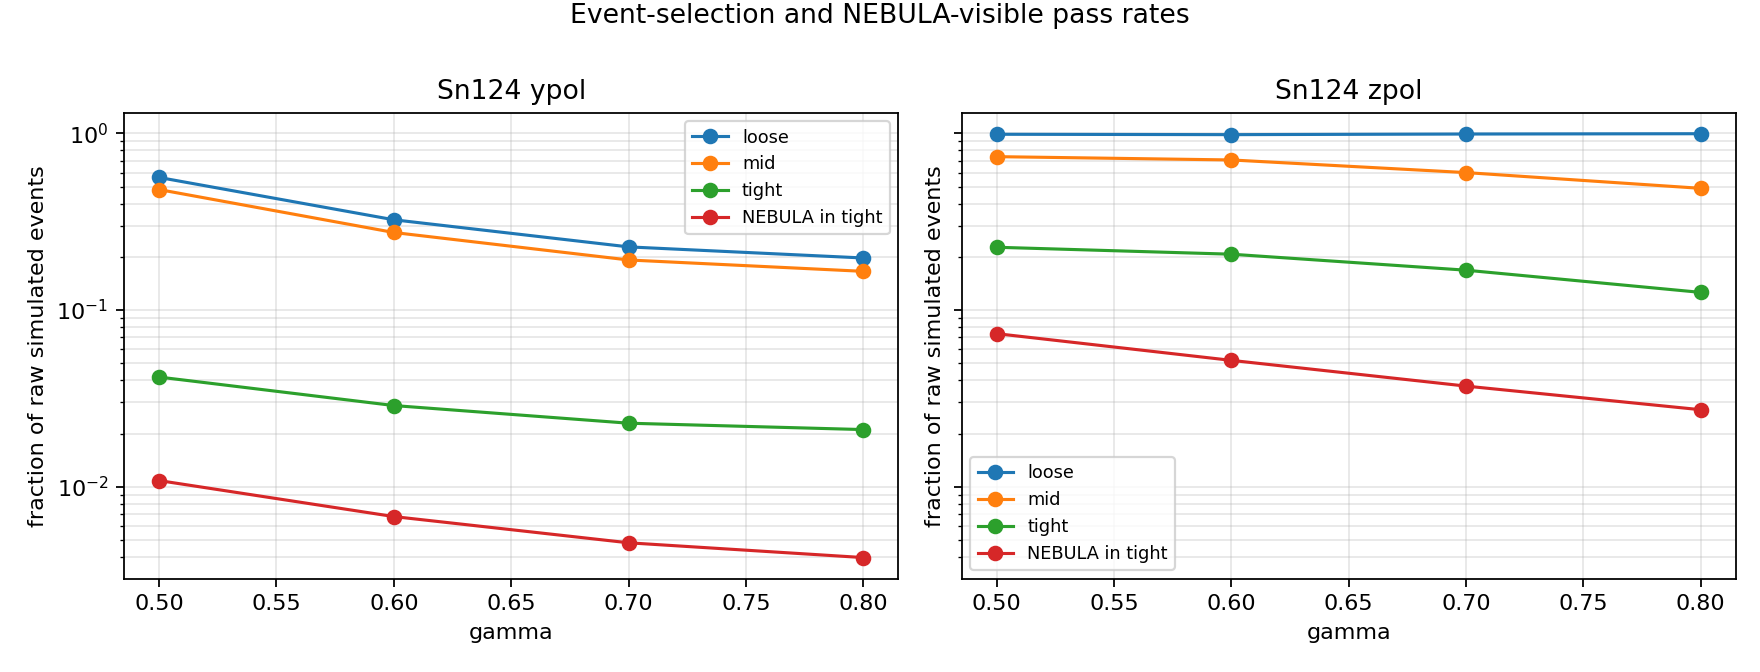
\includegraphics[width=0.96\linewidth]{sn124_selection_passrates.png}
  \caption{Sn124 selection pass rates versus $\gamma$. The final NEBULA-visible tight sample is the small fraction that can enter the folded $R$ observable.}
\end{figure}

For Sn124, the pooled y-pol sample has raw-to-tight and raw-to-NEBULA-visible fractions of about $2.59\%$ and $0.571\%$. The z-pol sample has larger fractions, about $16.1\%$ and $3.93\%$, because the generated and selected phase spaces are different. These numbers are used only as the simulation-derived useful-event survival factors; they are not a replacement for the experimental coincidence-efficiency calibration.

\begin{figure}[H]
  \centering
  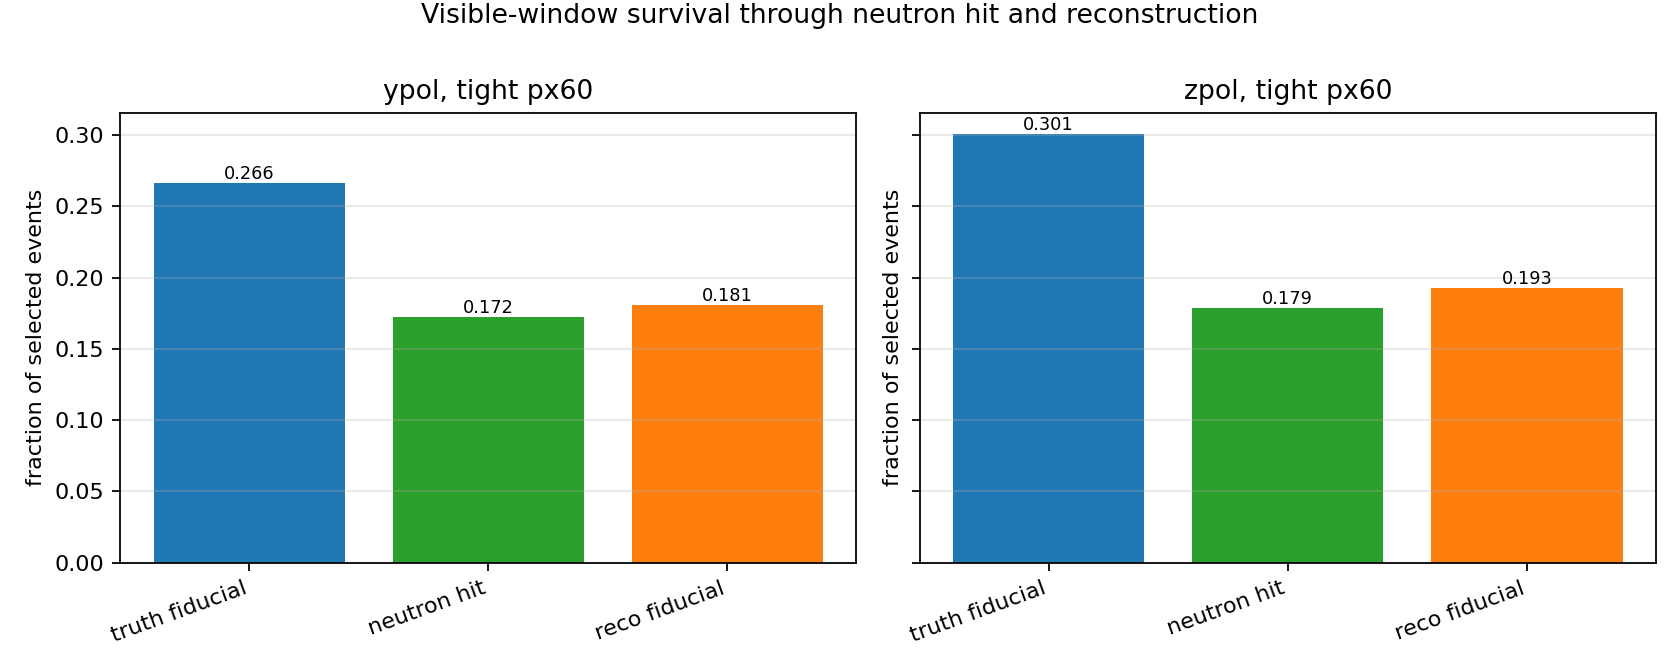
\includegraphics[width=0.95\linewidth]{survival_flow_tight_px60.png}
  \caption{Survival inside the tight px60 diagnostic sample. The truth fiducial fraction is set by the visible-window definition; the next steps show neutron hit and reconstructed-fiducial survival.}
\end{figure}

For pooled tight px60 events, y-pol keeps $0.266$ of selected events in the truth fiducial window, $0.172$ after neutron hit, and $0.181$ after reconstructed-fiducial selection. The corresponding z-pol fractions are $0.301$, $0.179$, and $0.193$. The reconstructed-fiducial count can be slightly above the hit-truth-fiducial count because the fiducial condition is applied after reconstruction and can migrate events across the boundary.

\subsection{Neutron efficiency in px-py and Delta-px phase space}

\begin{figure}[H]
  \centering
  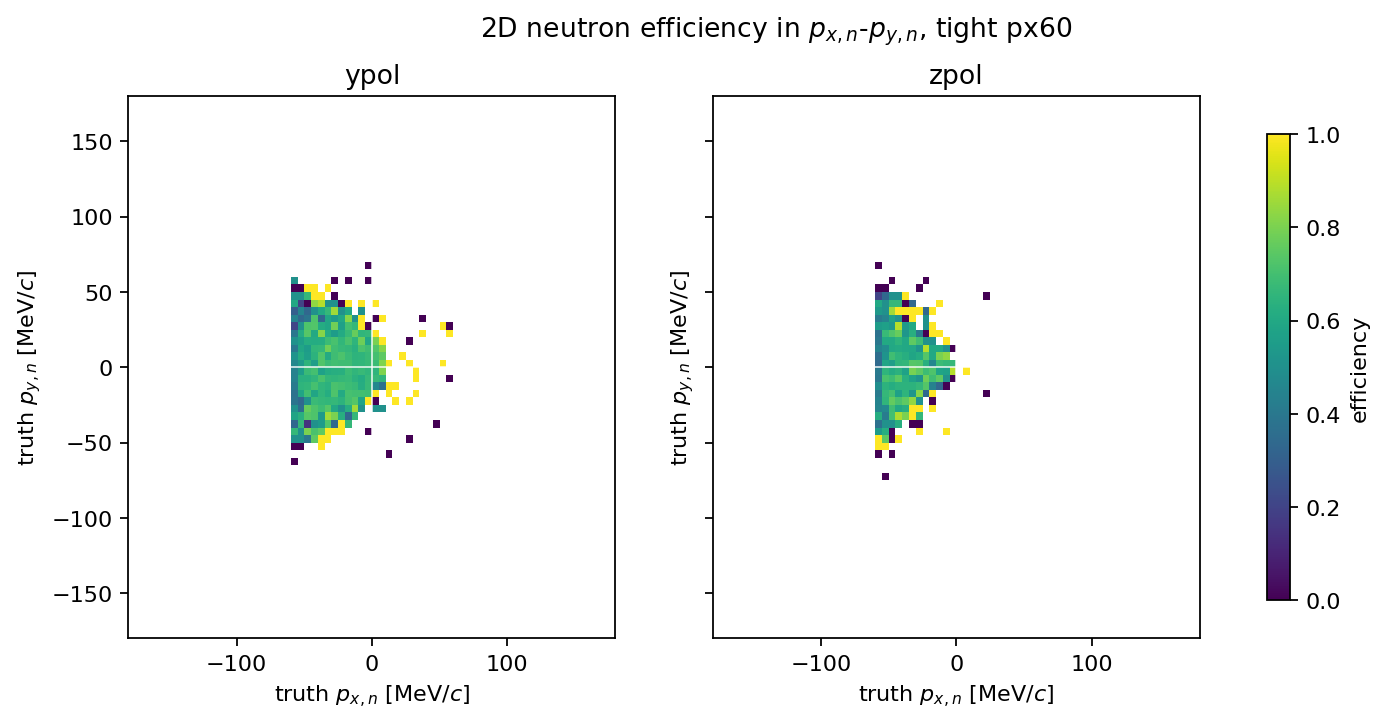
\includegraphics[width=0.96\linewidth]{neutron_efficiency_2d_pxn_vs_pyn_tight_px60.png}
  \caption{Two-dimensional neutron efficiency in truth $p_{x,n}$ versus truth $p_{y,n}$ for tight px60. Empty white regions are outside the populated/usable diagnostic phase space.}
\end{figure}

\begin{figure}[H]
  \centering
  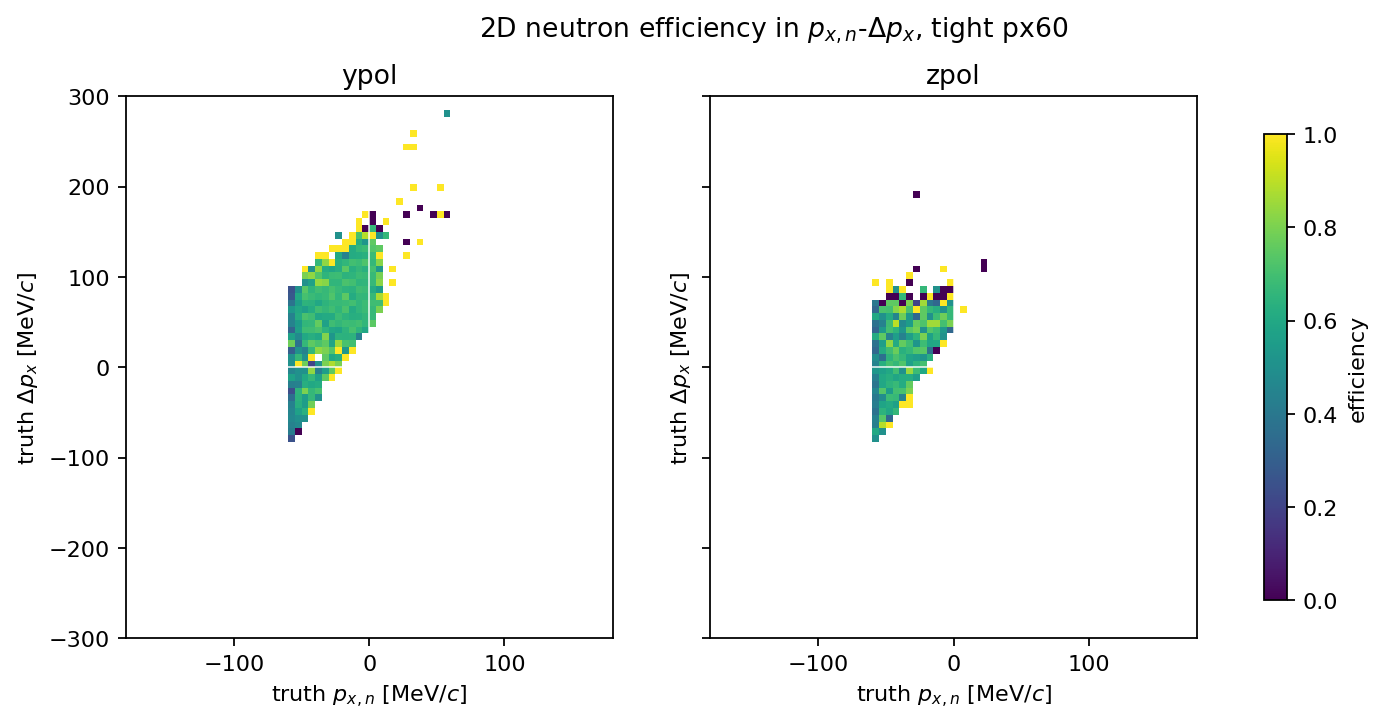
\includegraphics[width=0.96\linewidth]{neutron_efficiency_2d_pxn_vs_dpx_tight_px60.png}
  \caption{Two-dimensional neutron efficiency in truth $p_{x,n}$ versus truth $\Delta p_x$. This is the most direct efficiency map for the sign observable because it links neutron acceptance to the final numerator/denominator of $R$.}
\end{figure}

\begin{figure}[H]
  \centering
  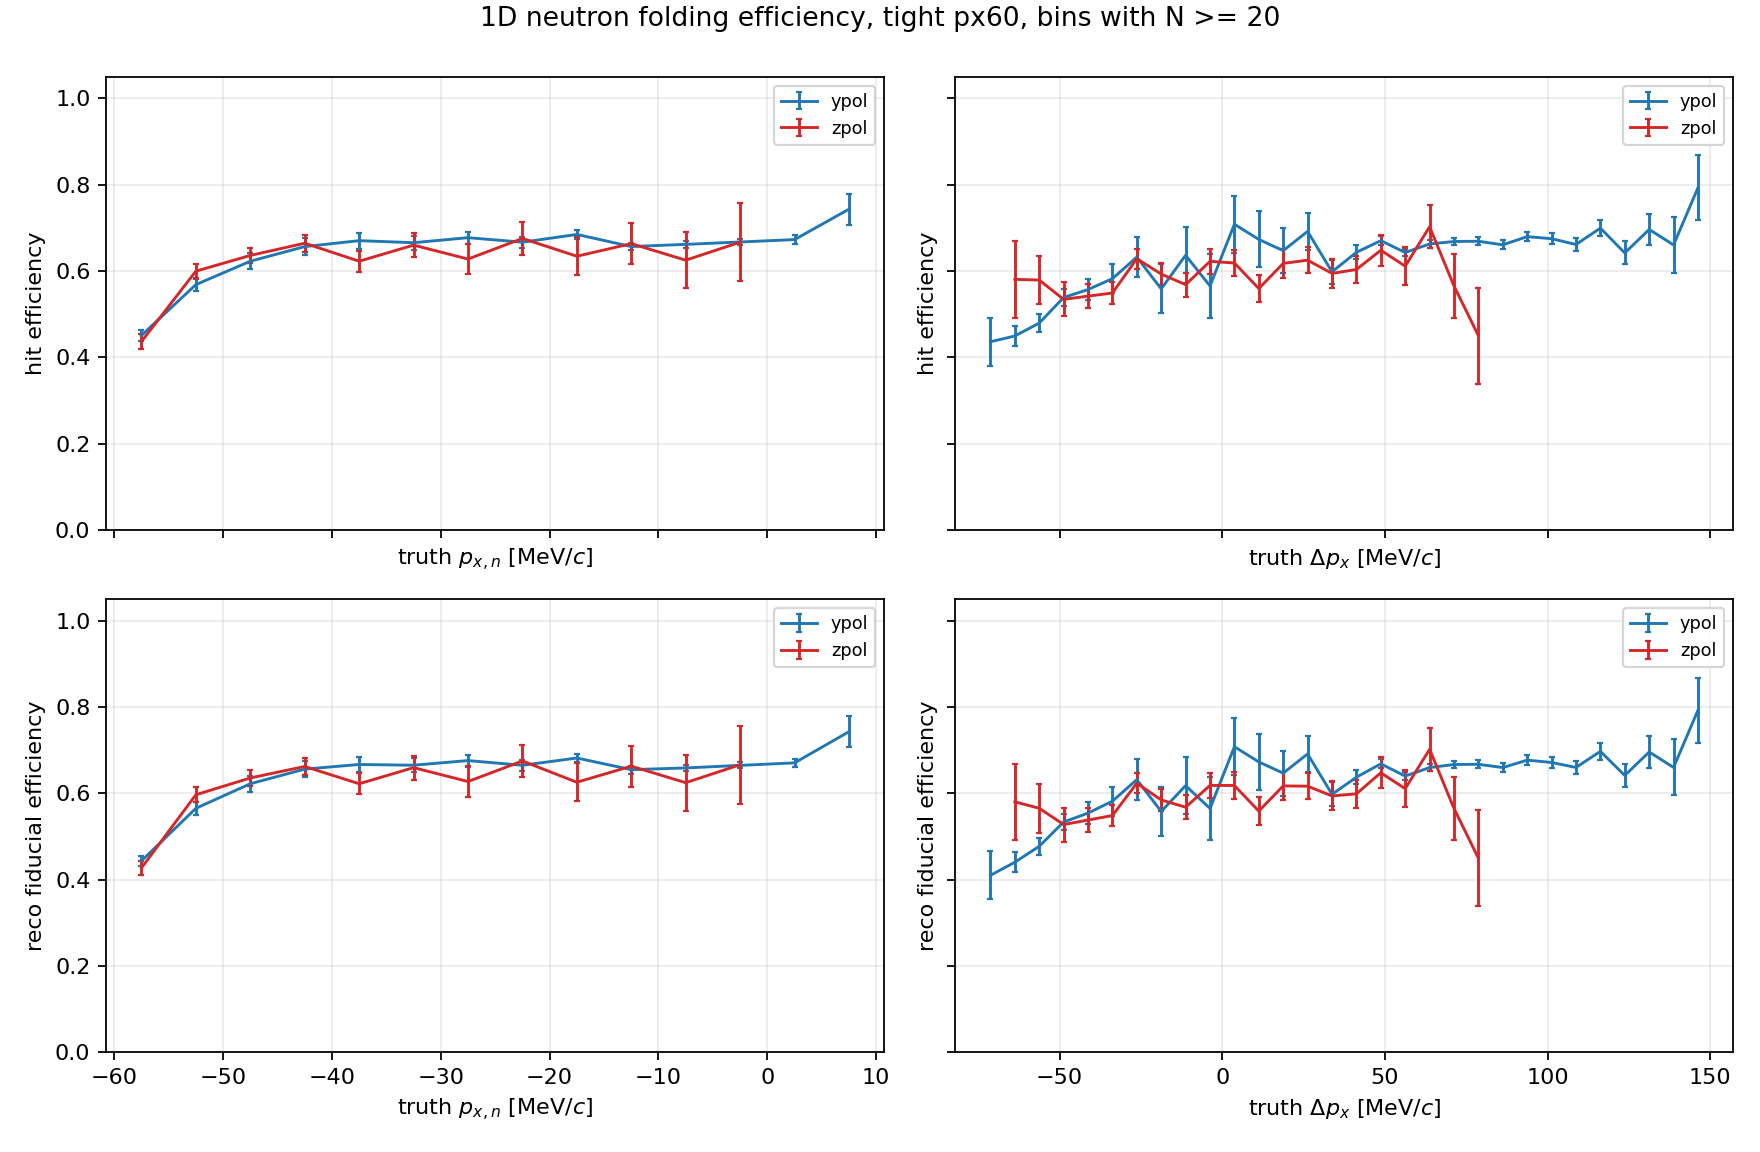
\includegraphics[width=0.96\linewidth]{neutron_efficiency_1d_tight_px60.png}
  \caption{One-dimensional neutron hit and reconstructed-fiducial efficiencies for bins with at least 20 truth events. In the populated core, the efficiency is typically around 0.55--0.70 rather than flat at unity.}
\end{figure}

The visible sample is not a uniform slice of the breakup phase space. The populated tight px60 region lies mostly at negative $p_{x,n}$, and the efficiency varies across both $p_{x,n}$ and $\Delta p_x$. This is exactly why the proposal should not claim that the measured $R$ directly equals the truth-level $R$. The defensible claim is that the same efficiency map can be applied to every simulated $\gamma$ point and tested with closure.

\subsection{Sign-dependent neutron efficiency and the px60 choice}

\begin{figure}[H]
  \centering
  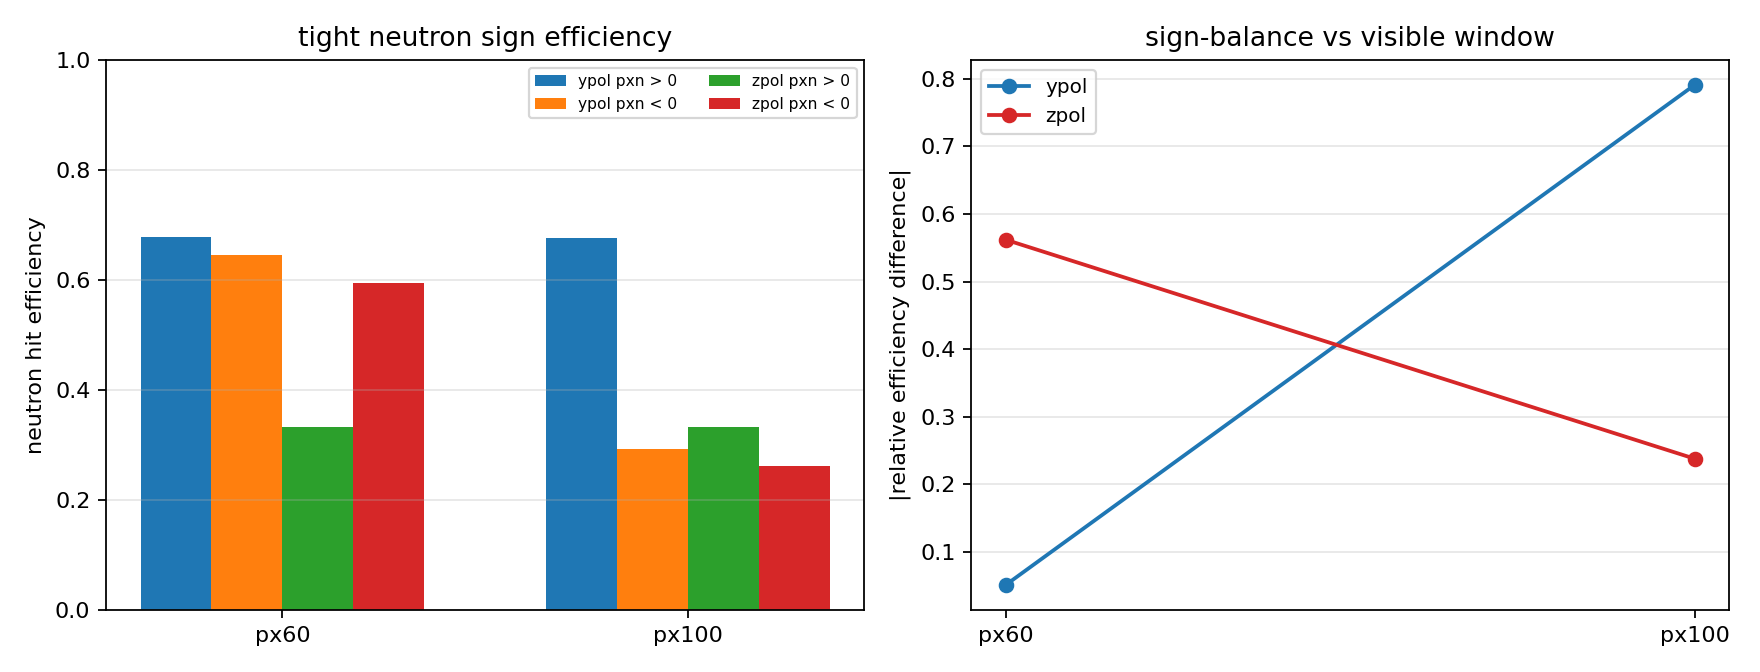
\includegraphics[width=0.95\linewidth]{ypol_tight_neutron_efficiency_balance.png}
  \caption{Neutron sign efficiency balance for tight selections. The y-pol sample gives the stable sign-balance comparison; z-pol tight has very small positive-$p_{x,n}$ statistics in this diagnostic.}
\end{figure}

For y-pol tight, the neutron hit efficiencies are:

\begin{table}[H]
\centering
\begin{tabular}{lrrr}
\toprule
fiducial & $\epsilon(p_{x,n}>0)$ & $\epsilon(p_{x,n}<0)$ & relative difference \\
\midrule
px60 & 0.678 & 0.644 & 0.050 \\
px100 & 0.677 & 0.293 & 0.791 \\
\bottomrule
\end{tabular}
\end{table}

The px100 selection retains a negative-$p_{x,n}$ branch that NEBULA sees very poorly, which strongly distorts $R$ through a sign-dependent detector efficiency. The px60 selection does not remove all detector effects, but it reduces the largest y-pol sign-dependent efficiency imbalance to a range that can be modeled and tested with closure studies. The current z-pol tight sign-balance number should not be over-interpreted because the positive-$p_{x,n}$ branch contains only three events in the current MC diagnostic table.

\subsection{Momentum and reaction-plane response}

\begin{figure}[H]
  \centering
  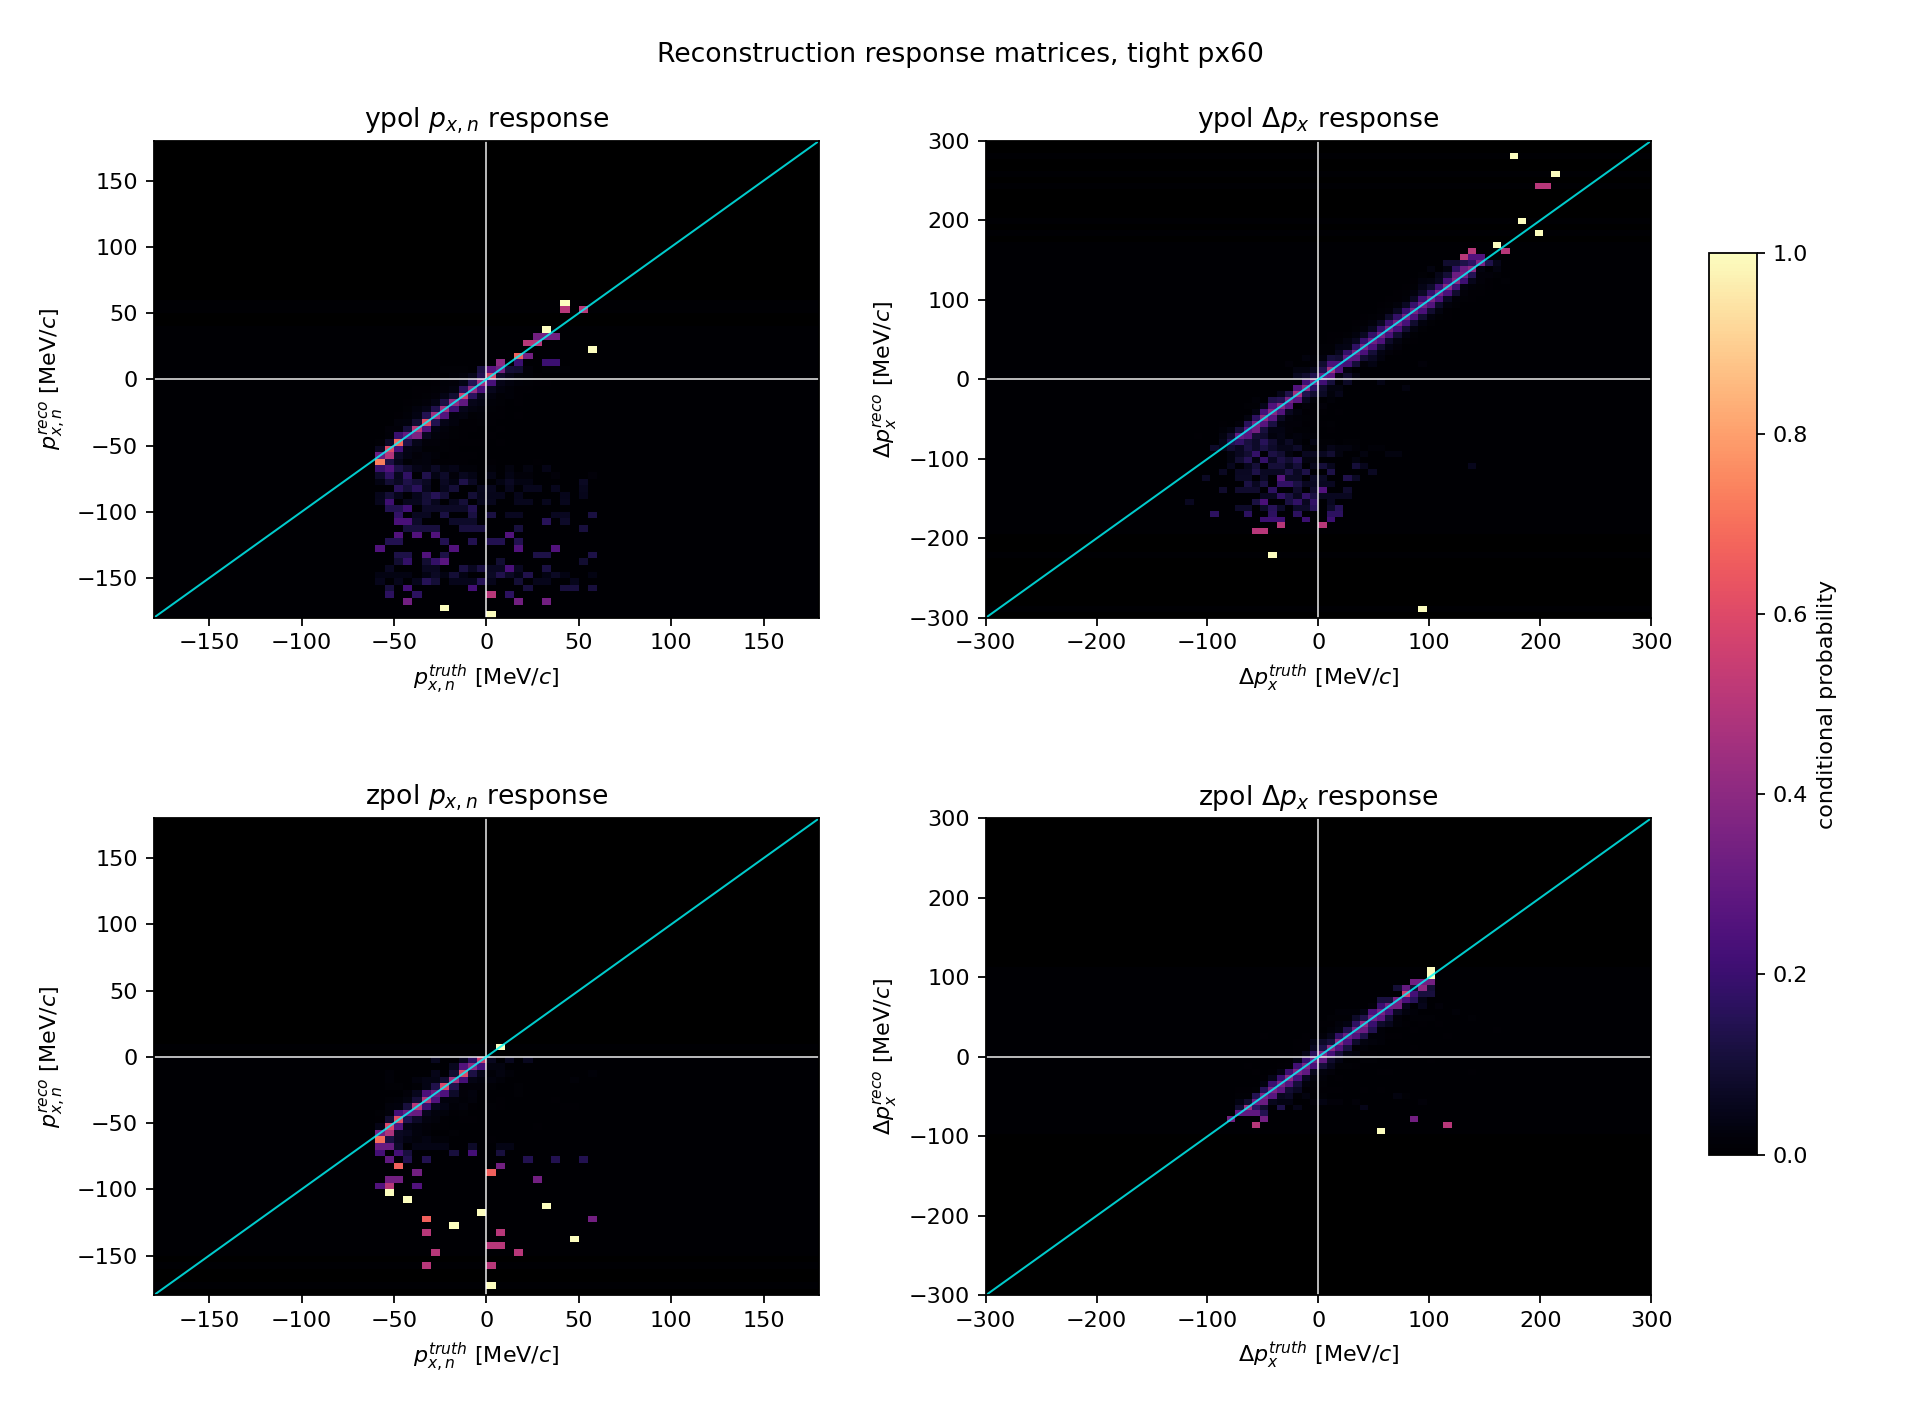
\includegraphics[width=0.96\linewidth]{response_matrices_tight_px60.png}
  \caption{Conditional response matrices for reconstructed $p_{x,n}$ and reconstructed $\Delta p_x$ in tight px60. The cyan line is the diagonal. Black regions are bins without usable diagnostic statistics.}
\end{figure}

The $\Delta p_x$ response is concentrated near the diagonal for both polarizations in the core region. The $p_{x,n}$ response is narrower in the accepted branch but also shows low-probability tails and boundary effects. This pattern supports the same conclusion as the efficiency maps: reconstruction smearing is relevant and must be folded, but the first-order bias in $R$ comes from which neutron kinematics enter the visible region.

\begin{figure}[H]
  \centering
  \begin{minipage}{0.48\linewidth}
    \centering
    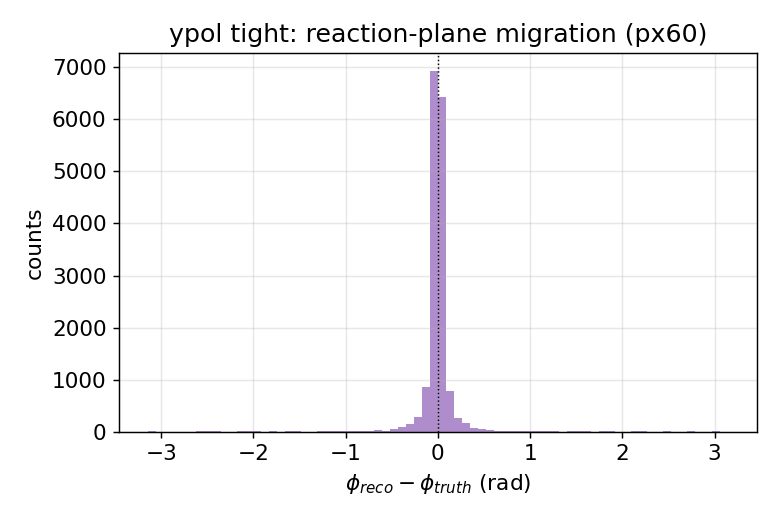
\includegraphics[width=\linewidth]{dphi_reco_truth_ypol_tight_px60.png}
  \end{minipage}
  \hfill
  \begin{minipage}{0.48\linewidth}
    \centering
    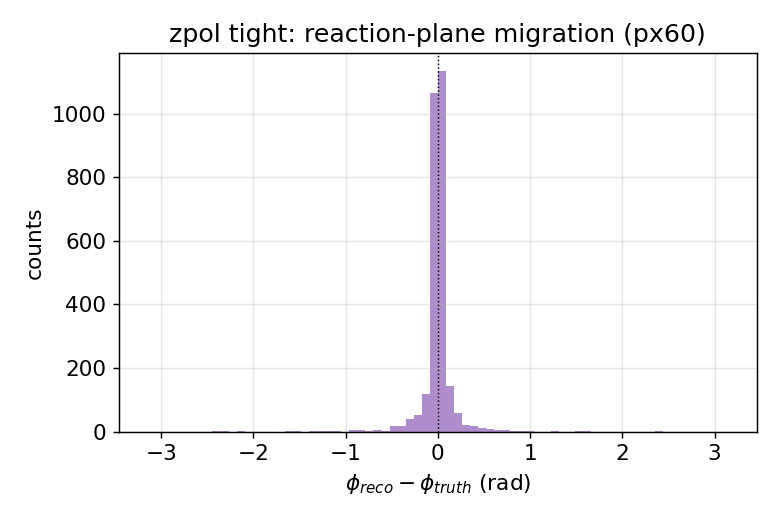
\includegraphics[width=\linewidth]{dphi_reco_truth_zpol_tight_px60.png}
  \end{minipage}
  \caption{Reconstructed minus truth reaction-plane angle for y-pol and z-pol tight px60. This is the direct diagnostic of the proton/PDC-driven event-plane reconstruction used by the $R$ observable.}
\end{figure}

\subsection{Where the folding changes R}

\begin{figure}[H]
  \centering
  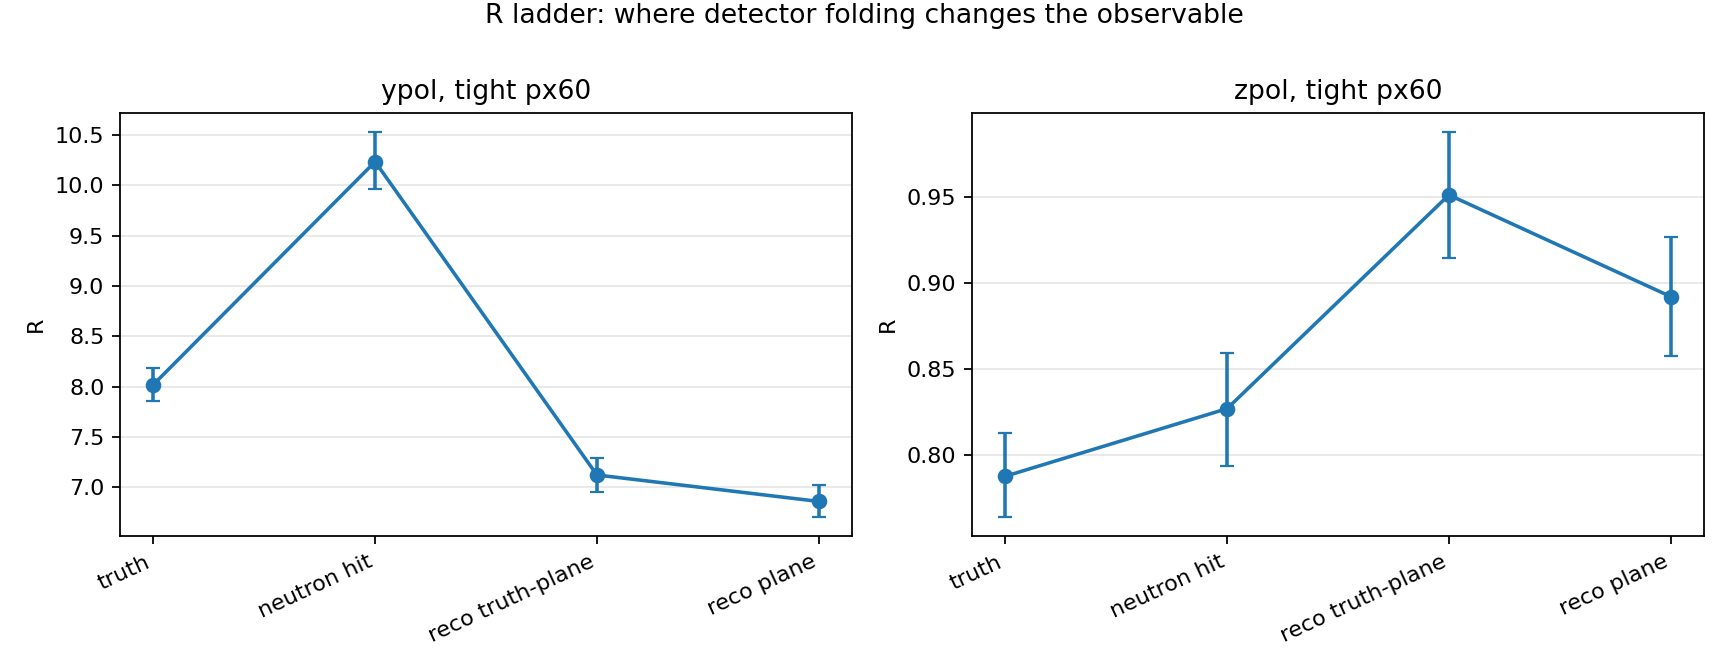
\includegraphics[width=0.96\linewidth]{r_ladder_summary_tight_px60.png}
  \caption{$R$ ladder for y-pol and z-pol tight px60. The ladder separates truth, neutron-hit acceptance, truth-plane reconstruction, and fully reconstructed event-plane effects.}
\end{figure}

For pooled y-pol tight px60:

\begin{table}[H]
\centering
\begin{tabular}{lrrrr}
\toprule
stage & $N$ & $N_{\mathrm{pos}}$ & $N_{\mathrm{neg}}$ & $R$ \\
\midrule
truth & 24323 & 21626 & 2697 & 8.02 \\
hit\_truth & 15751 & 14349 & 1402 & 10.23 \\
reco\_truth\_plane & 16509 & 14476 & 2033 & 7.12 \\
reco\_plane & 16509 & 14408 & 2101 & 6.86 \\
\bottomrule
\end{tabular}
\end{table}

The largest visible change happens before the final event-plane reconstruction: neutron hit acceptance and the reconstructed visible-window definition move the observable substantially. The smaller change from \texttt{reco\_truth\_plane} to \texttt{reco\_plane} shows that the PDC/reaction-plane reconstruction is not the dominant $R$-bias term in the current diagnostic sample.

\subsection{Sign migration is not the leading effect}

\begin{figure}[H]
  \centering
  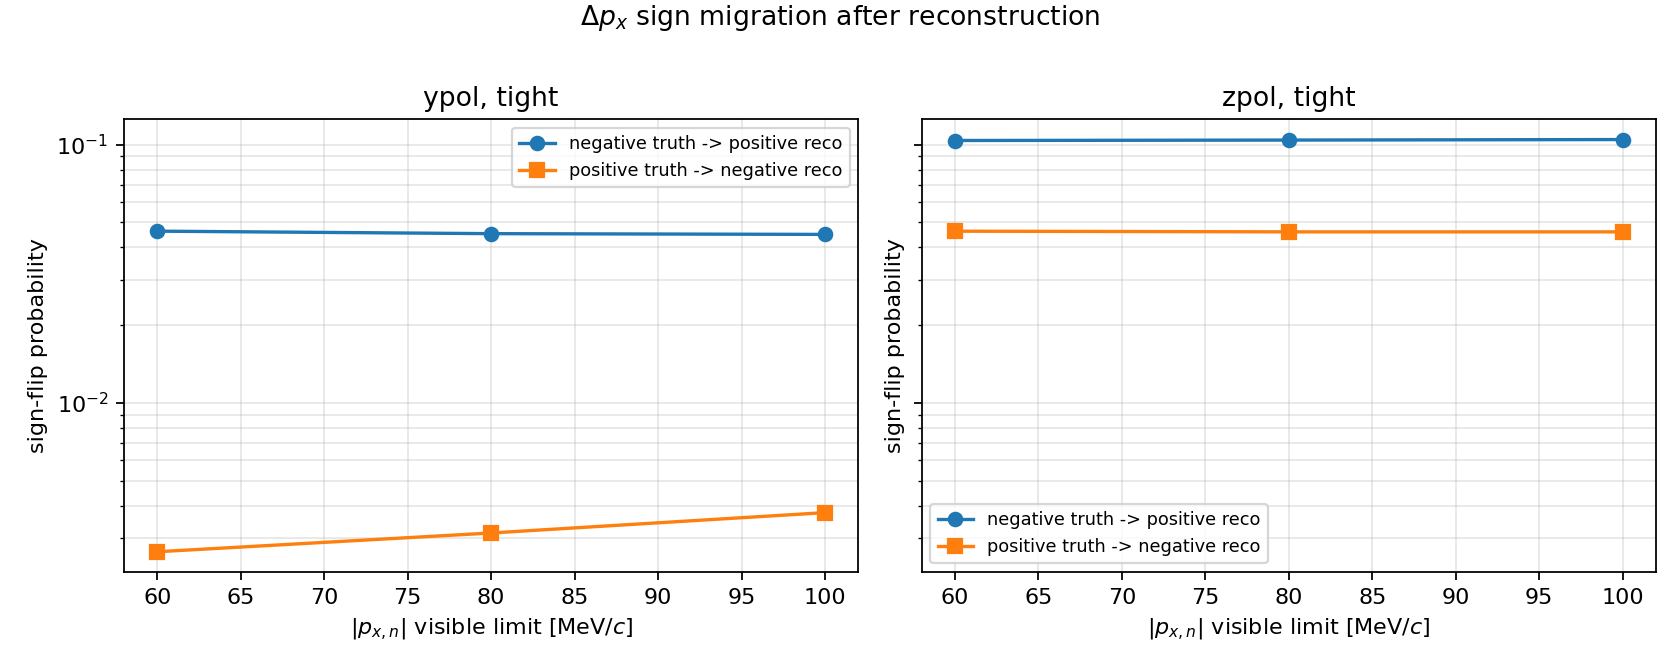
\includegraphics[width=0.95\linewidth]{sign_migration_summary_tight.png}
  \caption{$\Delta p_x$ sign-flip probability versus neutron visible-window size for tight selections.}
\end{figure}

For tight px60, the sign-migration probabilities are:

\begin{table}[H]
\centering
\begin{tabular}{llrr}
\toprule
polarization & truth sign & $P(\mathrm{reco\ negative})$ & $P(\mathrm{reco\ positive})$ \\
\midrule
y-pol & negative & 0.954 & 0.046 \\
y-pol & positive & 0.00265 & 0.997 \\
z-pol & negative & 0.896 & 0.104 \\
z-pol & positive & 0.046 & 0.954 \\
\bottomrule
\end{tabular}
\end{table}

Within the visible window, sign flipping of $\Delta p_x$ is therefore not the main uncertainty. The leading issue is still which neutron kinematics enter the visible and reconstructable phase space.

\section{Statistics and Beam Time}

The current beamtime planning anchor is:
\begin{itemize}
  \item beam energy: 190 MeV/u
  \item beam intensity: $1.0\times10^7$ pps
  \item SRC harmonic number: 6
  \item bunch spacing: 33.62 ns
  \item planning breakup cross section: 550 mb
  \item planning detected-coincidence efficiency: 4.65\%
\end{itemize}

For the 15 mm Sn124 target option under the 1.2 g inventory constraint:
\begin{itemize}
  \item equivalent thickness: 0.929 mm
  \item detected coincidence rate: 843 Hz
  \item detected coincidences in 16 h: $4.86\times10^7$
\end{itemize}

After applying the conservative usable-event survival from the current full simulation:

\begin{table}[H]
\centering
\begin{tabular}{lrrr}
\toprule
polarization & useful fraction & 16 h usable $R$ events & worst adjacent-$\gamma$ 3$\sigma$ $N$ \\
\midrule
y-pol & 0.00566 & $2.75\times10^5$ & $2.77\times10^3$ \\
z-pol & 0.03869 & $1.88\times10^6$ & $1.31\times10^2$ \\
\bottomrule
\end{tabular}
\end{table}

\begin{figure}[H]
  \centering
  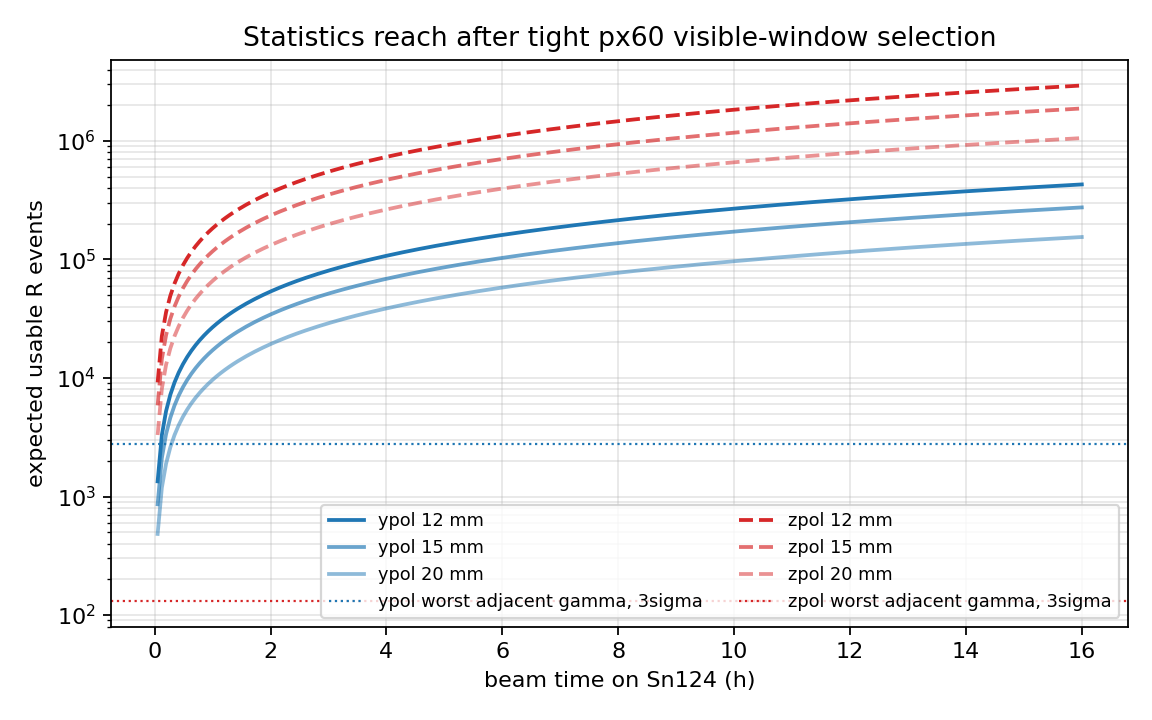
\includegraphics[width=0.9\linewidth]{sn124_beamtime_reach_tight_px60.png}
  \caption{Usable $R$-event reach after the tight px60 visible-window selection for the Sn124 inventory target options.}
\end{figure}

Even with the 20 mm disk option, still using the same 1.2 g Sn inventory, the expected y-pol usable $R$ events after 16 h remain above $10^5$. The experiment is statistically capable of constraining $\gamma$ in this folded-observable strategy. The final uncertainty budget will be controlled by detector response, neutron efficiency, and model-folding systematics.

For pile-up, the older 3 mm reference thickness gives a detected-coincidence mean of about $9.16\times10^{-5}$ per bucket. The 15 mm inventory option has a lower rate, so single-bucket pile-up is not the main limitation. The electronics integration window still needs to be checked for possible multi-bucket pile-up.

\section{Recommended Gamma-Constraint Workflow}

The recommended analysis path is:
\begin{enumerate}
  \item For each QMD $\gamma$ point, run the same Geant4 geometry, NEBULA-Plus detector response, PDC NN proton reconstruction, and neutron reconstruction.
  \item Define the same folded observable for data and model: the tight event selection plus $|p_{x,n}^{\mathrm{reco}}|<60$ MeV/$c$, with Sn124 as the primary target.
  \item Construct the experimental observable
  \[
    R_{\mathrm{exp}}
    =
    \frac{N(\Delta p_x^{\mathrm{reco}}>0)}
         {N(\Delta p_x^{\mathrm{reco}}<0)}.
  \]
  \item Construct the folded model prediction $R_{\mathrm{model,folded}}(\gamma)$.
  \item Use a likelihood or $\chi^2$:
  \[
    \chi^2(\gamma)
    =
    \frac{
      \left[
        R_{\mathrm{exp}} - R_{\mathrm{model,folded}}(\gamma)
      \right]^2
    }{
      \sigma_{\mathrm{stat}}^2
      + \sigma_{\mathrm{detector}}^2
      + \sigma_{\mathrm{model}}^2
    }.
  \]
  \item Combine y-pol/z-pol and Sn112/Sn124 only after each channel has its own closure test and systematic uncertainty estimate. Do not combine channels using statistical errors alone.
\end{enumerate}

This route avoids an unstable unfolding problem. An unfolded truth-level $R$ should be treated as an additional result only if closure tests demonstrate that the response matrix is sufficiently constrained and that near-zero-efficiency regions are not driving the result.

\section{Remaining Work}

The current report should not overstate the following points:
\begin{itemize}
  \item $\eta_{\mathrm{coin}}=4.65\%$ is still a manuscript planning anchor. The local selected-breakup validation reproduces an acceptance of about 37.9\%. These are different definitions and must be kept separate in the proposal.
  \item Target-specific Sn112 and Sn124 breakup cross sections still need a consistent ImQMD shell-integration extraction. They should not be obtained by simply rescaling the Sn124 anchor.
  \item Real-data neutron efficiency calibration, timing offsets, thresholds, cross-talk, fake neutrons, and accidental backgrounds are not yet included.
  \item The detector-response systematic uncertainty has not yet been quantified with toy closure or pseudo-data closure tests.
  \item The current diagnostic report uses a mixture of simulation truth-defined event cuts and a reconstructed visible-window definition. The final experimental analysis should express all data-side cuts in reconstructed quantities, with simulation truth used only for validation and interpretation.
\end{itemize}

\section{Recommended Proposal Wording}

The defensible statement is:
\begin{quote}
For Sn124, after NEBULA-Plus detector response, PDC NN proton reconstruction, and neutron reconstruction, the folded $R$ observable with the tight event selection and $|p_{x,n}|<60$ MeV/$c$ retains a strong $\gamma$ dependence. Under the current 15 mm/1.2 g Sn target option, $1.0\times10^7$ pps beam intensity, and 16 h planning assumption, the expected statistics exceed the 3$\sigma$ adjacent-$\gamma$ separation requirement by roughly two orders of magnitude. The feasibility of constraining $\gamma$ is therefore controlled mainly by detector-folding systematics, not by raw statistics.
\end{quote}

The following statement should not be used:
\begin{quote}
The reconstructed $R$ is already equal to the truth-level $R$.
\end{quote}

The more accurate statement is:
\begin{quote}
The experiment should compare folded data with folded model predictions. The truth-level $R$ should be used as a physics interpretation and closure-test reference.
\end{quote}

\end{document}
